\section{Red laboral}
Para explorar nuevas topologias y relaciones se decidi'o monitorear una red laboral en una oficina de mediana envergadura. En esta
red local conviven computadoras de empleados, servidores de distinto uso, impresoras de red y otros dispositivos de oficina. 

El primer experimento, en el cual se ve la red como una fuente con 2 s'imbolos unicamente (Unicast y Broadcast), monitore'o la red local 
a trav'es de un enlace
Ethernet durante 20 minutos. Como era de esperarse cerca del 100\% del tr'afico es unicast dado que es una red con mucho tr'afico
hacia un servidor en particular o hacia el gateway.

\begin{figure}[!h]
\centering
\caption{Informaci'on de S, Red laboral}
\begin{tabular}{ r|c|c| }
\multicolumn{1}{r}{}
 &  \multicolumn{1}{c}{frecuencia}
 & \multicolumn{1}{c}{informaci'on} \\
\cline{2-3}
$S_{broadcast}$ & 0.03 & 5.06 \\
\cline{2-3}
$S_{unicast}$ & 0.97 & 0.04 \\
\cline{2-3}
\end{tabular}
\end{figure}
 
 Estos valores nos dan una entrop'ia de 0.19 bits (siendo el m'aximo 1 dado que hay 2 simbolos en principio equiprobables),
 dado que el tr'afico broadcast sin ser despreciable s'olo es un porcentaje peque\~no del tr'afico total.\\
 
En el segundo experimento, el cual modela la red basado en la direcci'on a resolver en mensajes ARP, usamos la misma captura
utilizada en el experimento anterior. Bajo nuestra definici'on para destacar nodos (que la informaci'on del simbolo de ese nodo 
sea menor o igual a la entrop'ia de la fuente) s'olo un nodo fue destacado por amplio margen, el gateway por defecto de la red.\\

\begin{figure}[!h]
\centering
\caption{Informaci'on red laboral}
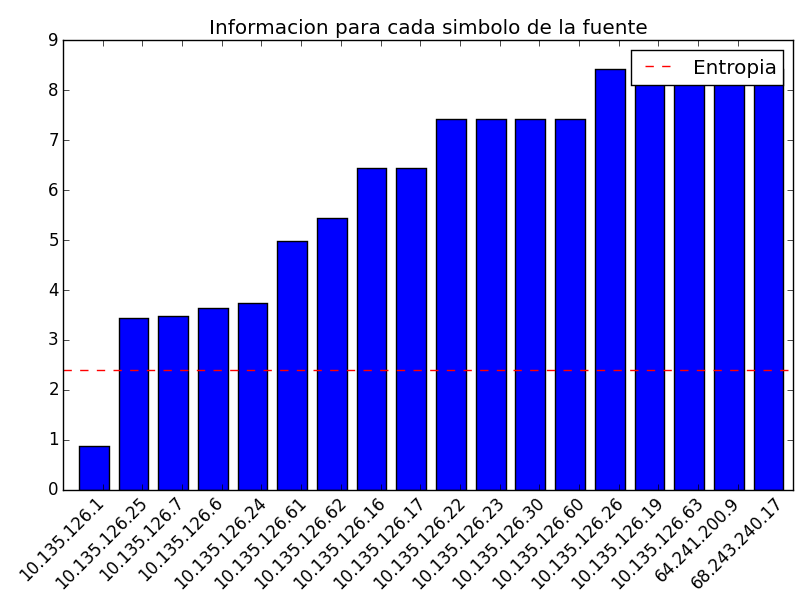
\includegraphics[width=0.55\textwidth]{red2_info}
 \label{fig:red2info}
\end{figure}

La visualizaci'on de la red modelada como la fuente descriptiva muestra una topologia y relaci'on entre nodos muy similar
a la realidad en t'erminos de trafico total y disposici'on.


Un an'alisis manual del tr'afico evidenci'o dos fen'omenos ARP no usuales, ARP gratuitos y ARP de sondeo. Los ARP gratituitos pueden
ser tanto \texttt{who-has} como \texttt{is-at} donde tanto la direcci'on de origen como la direcci'on de destino son las mismas (y la direcci'on
de enlace destino es broadcast). El uso de los mismos es precargar o refrescar las tablas de otros nodos para evitar tener
que traducir en tiempo real una direcci'on de red. Los ARP de sondeo tienen un fin similar, un nodo al que se le asign'o manualmente
o automaticamente una direcci'on de red, envia un ARP con dicha direcci'on a la red y si alg'un nodo le responde entonces sabr'a
que la direcci'on ya est'a en uso y evitar'a as'i la colisi'on de alguna forma. Ninguno de estos tipos de mensajes est'an oficialmente
documentados pero forman parte de toda red que necesite autoregularse correctamente.\\

\begin{figure}[!h]
\centering
\caption{Visualizaci'on red laboral, en amarillo los nodos destacados}
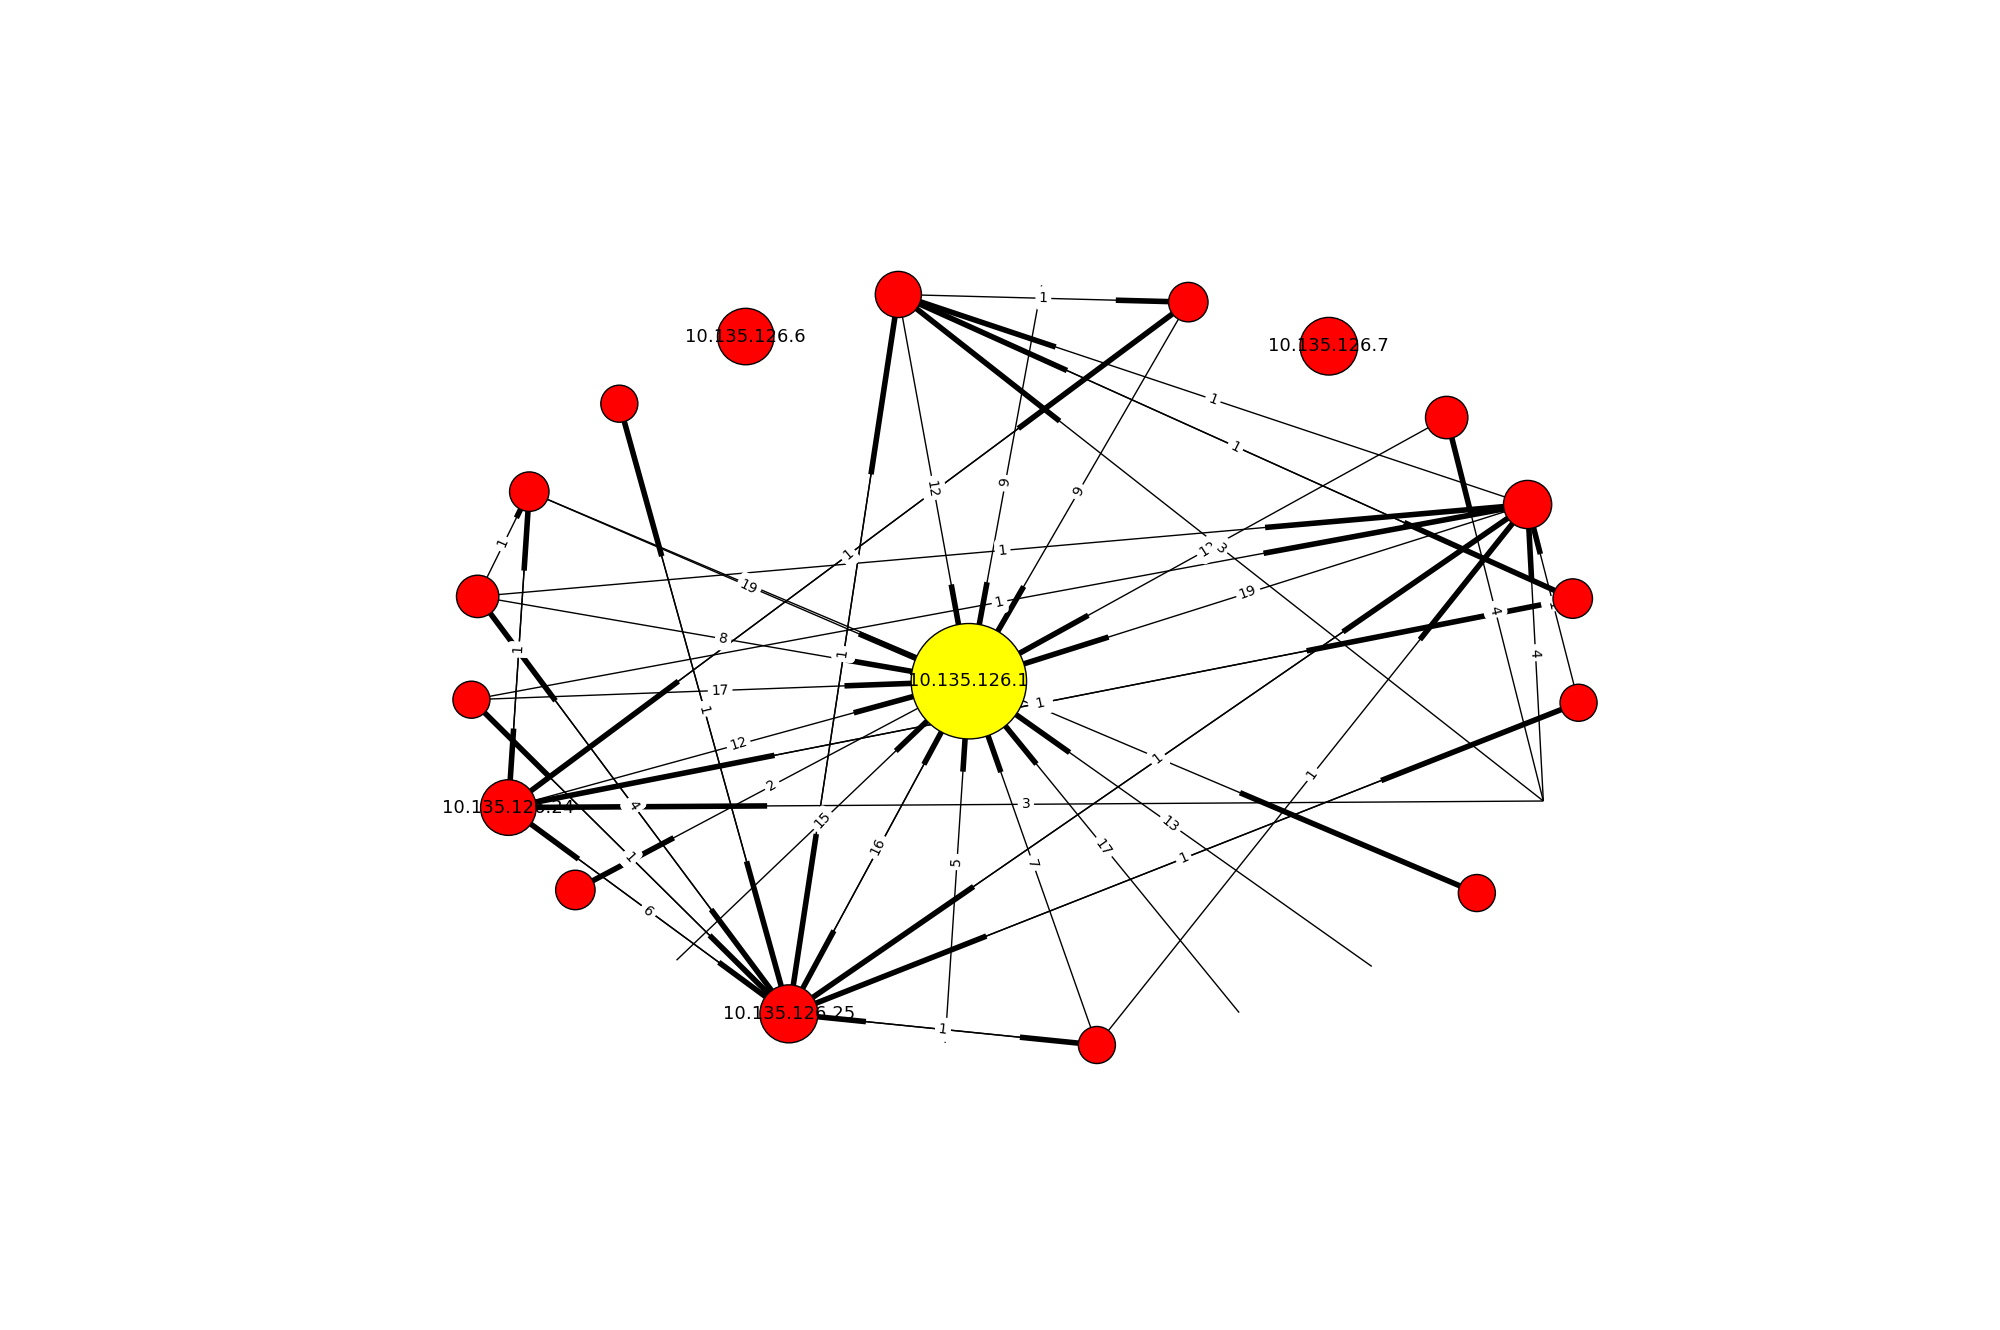
\includegraphics[width=0.9\textwidth]{red2_red}
 \label{fig:red2net}
\end{figure}